\subsection*{Introduzione teorica}

Si vuole studiare il problema agli autovalori:
$$ \Hh\psi = E \psi $$
%
Siano $k^2 = 2E$ e  $q^2 = 2(E-V0)$. La soluzione analitica più generale è data da:
%
$$
\psi_k(x) =
    \begin{cases}
        Ae^{ikx}+Be^{-ikx} & \mbox{in ZonaI} \\
        \phi(x) & \mbox{in ZonaII} \\
        Ce^{ikx}+De^{-ikx} & \mbox{in ZonaIII} \\
    \end{cases}
$$
%
\bigskip
Non siamo per il momento interessati alla ZonaII, quindi indichiamo con
$\phi(x)$ la $\psi_k(x)$ in tale zona, che a rigore sarebbe
    $$\phi(x)= Ee^{iqx}+Fe^{-iqx}$$
Le costanti $A,B,C,D$ sono determinate dalle condizioni di raccordo di continuità della
funzione d'onda e della sua derivata nei punti $x=\pm b$.\\
Si osserverà che dalla diagonalizzazione della versione discreta della Hamiltoniana
(vedi sezione apposita) risultano autofunzioni a parità definita (pari o dispari).
Il problema consiste in due onde una progressiva e una regressiva, che perturbate
dalla barriera vengono entrambe riflesse e trasmesse e interferiscono l'una con
l'altra e con se stesse.
Per la simmetria del problema, il coefficiente di riflessione e di trasmissione
relativi all'onda progressiva e quella regressiva sono gli stessi.
Si può allora parametrizzare ciascuna onda come:
    $$ Ae^{ikx} + Be^{-ikx} = Ae^{ikx} + A(\rho + \tau)e^{-ikx} $$
Dove $\rho$ e $\tau$ sono i coefficienti il cui modulo quadro dà, rispettivamente
il coefficiente di riflessione e trasmissione.
In forma matriciale:
$$
    \begin{pmatrix} C \\ B \end{pmatrix} =
    \begin{pmatrix} \tau & \rho \\ \rho & \tau \end{pmatrix} \cdot
    \begin{pmatrix} A \\ D \end{pmatrix} = \quad (S)\cdot \begin{pmatrix} A \\ D \end{pmatrix}
$$
%
Ove la matrice S è una matrice unitaria, che di conseguenza verifica le condizioni:
$$ \tau\rho^* + \tau^*\rho = 0 \quad,\quad |\tau|^2 + |\rho|^2 = 1$$
(Si è indicato con $z^*$ il numero complesso coniugato di $z$). Segue immediatamente che:
$$ |\tau \pm \rho|^2 = |\tau|^2 + |\rho|^2 + \tau\rho^* + \tau^*\rho = |\tau|^2 + |\rho|^2 + 0 = 1$$
Cioè $\tau \pm \rho$ differiscono per una fase:
$$ |\tau \pm \rho|^2 = 1 \Rightarrow (\tau \pm \rho) = e^{2i\theta^\pm}$$
%
Allora, senza perdita di generalità, si pone la ulteriore condizione di simmetria alle $\psi_k$, che porta:
$$\begin{cases}
    A = D, \qquad  B = C = (\tau + \rho)A &\mbox{per funzioni pari} \\
    A = -D, \quad B = -C = -(\tau + \rho)A &\mbox{per funzioni dispari}\\
\end{cases}$$
%
Si osservi che poichè $A,B,C,D$ dipendono dagli autostati $\psi_k$, anche le fasi $\theta^\pm$ dipenderanno dall'autovalore $k$.\\
Si vuole quindi cercare una stima numerica di $\theta\pm$ per determinare $\tau$ da:
    $$ (\tau \pm \rho) = e^{2i\theta^\pm} \Rightarrow \tau = 1/2(e^{2i\theta^+}+e^{2i\theta^-})$$
    $$ \Rightarrow \tau^2 = \sin^2(\theta^+ - \theta^-)$$
%(due conti per dimostrarlo plis) (OCCHIO che esce un coseno)
\\
Il coefficiente di trasmissione sarà qundi dato da:
    $$T = \tau^2$$

\subsection*{Stima delle Fasi}
Si vuole stimare numericamente le fasi $\theta^\pm$, a partire dagli autovettori
calcolati dalla $\Hh$ discretizzata. Gli autovettori sono combinazioni pari e dispari
di onde piane con la stessa frequenza, quindi corrispondono rispettivamente a coseni e seni.
    $$ \psi_k^{odd} = \begin{cases}
        A\sin(kx + \theta^-_k) & \mbox{in ZonaI} \\
        A\sin(kx + \theta^+_k) & \mbox{in ZonaIII} \\
    \end{cases}
    \quad
    \psi_k^{even} = \begin{cases}
        A\cos(kx + \theta^-_k) & \mbox{in ZonaI} \\
        A\cos(kx + \theta^+_k) & \mbox{in ZonaIII} \\
    \end{cases}
    $$
 \smallskip

\begin{paragraph}{Metodo:}
Si considerino gli autostati della Hamiltoniana
$$ \psi_k^{odd} = \begin{cases}
    A\sin(kx + \theta^-_k) & \mbox{in ZonaI} \\
    A\sin(kx + \theta^+_k) & \mbox{in ZonaIII} \\
\end{cases}
\quad
\psi_k^{even} = \begin{cases}
    A\cos(kx + \theta^-_k) & \mbox{in ZonaI} \\
    A\cos(kx + \theta^+_k) & \mbox{in ZonaIII} \\
\end{cases}
$$
Si pongano ora le condizioni di periodicità ai bordi della scatola $x = \pm L$
    $$  \psi_k^{odd}(L) = \psi_k^{odd}(-L) \quad,\quad \psi_k^{even}(L) = \psi_k^{even}(-L)$$
che portano a:
$$ A\sin(-kL + \theta^-_k) = A\sin(kL + \theta^+_k) \Rightarrow -kL + \theta^-_k = kL + \theta^+_k + 2n\pi $$
$$ A\cos(-kL + \theta^-_k) = A\cos(kL + \theta^+_k) \Rightarrow -kL + \theta^-_k = kL + \theta^+_k + 2n\pi $$
ossia,
      $$ \theta^-_k - \theta^+_k = 2kL + 2n\pi $$
quindi il coefficiente di trasmissione risulta essere:
    $$ T(k) = \tau^2(k) = \sin^2(\theta_k^+ - \theta_k^-) = \sin^2(\theta_k^- - \theta_k^+) = \sin^2(2kL + 2n\pi) $$
    $$ T = \sin^2(2kL) $$
\end{paragraph}

%
\newpage
\subsection*{Risultati}
Di seguito il plot del coefficiente di trasmissione calcolato numericamente contro
il risultato analitico

%% Immagine da mettere sotto la frase, possibilmente in una unica pagina - FATTO
\begin{figure}[h]
\centering
  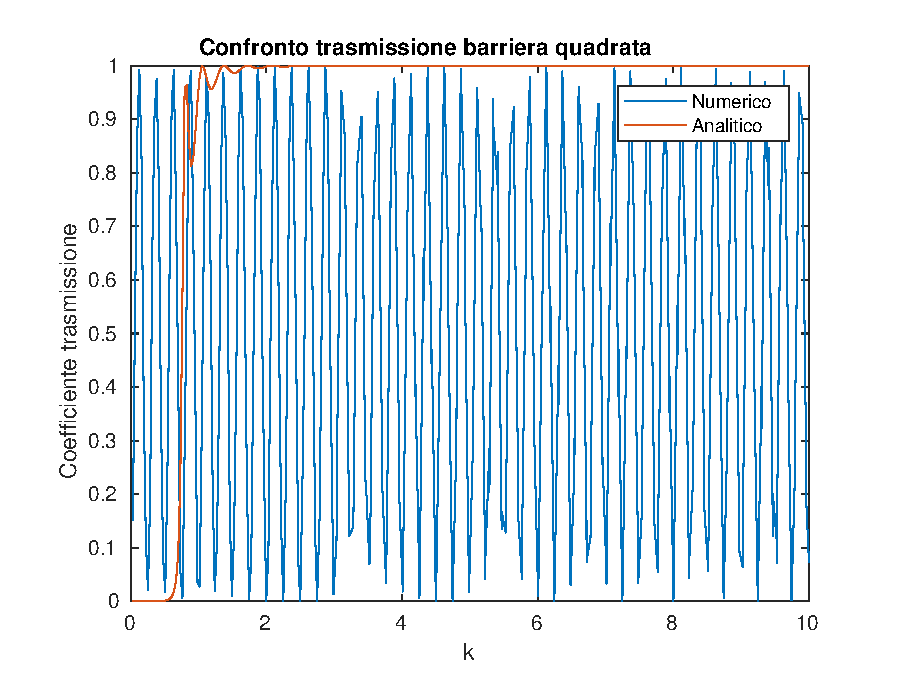
\includegraphics[width=10cm]{tr_coeff_square.eps}
\end{figure}
